\documentclass[12pt,a4paper]{article}
\pagestyle{plain}
\usepackage{fullpage}
\usepackage[english]{babel}
\usepackage{enumerate}

%equations
\usepackage[fleqn]{amsmath}
\numberwithin{equation}{section}

%figures
\usepackage[dvips]{graphicx}
\graphicspath{{./images/}}
\numberwithin{figure}{section}

%excercises
\newcounter{Exercise}
\setcounter{Exercise}{1}
\usepackage[dvipsnames]{xcolor}
\usepackage{framed}
\definecolor{shadecolor}{gray}{0.9}
\usepackage{caption}

%tables
\numberwithin{table}{section}

%specials
\usepackage{textcomp} %special (greek) characters as text
%\usepackage{pstricks} %
%\usepackage{ifthen} %
%\usepackage{calc} %
%\usepackage{isotope}
\usepackage{hyperref}
\usepackage[bottom]{footmisc} %footnote below figure
\usepackage{footnpag}%number footnotes per page


%document details
\author{N.G. Schultheiss \\ translated and adapted by K. Schadenberg}
\date{}
\title{The HiSPARC Detector}

%DIT IS DE NL TEKST DETECTEREN - NIET DETECTOR


\begin{document}
\maketitle

\section{Introduction}
The detectors used by the HiSPARC project are designed in such a way that they are sensitive to the particles created by cosmic rays. The heart of the detector is a 1.0~m by 0.5~m scintillating plate. This plate converts the energy of particles passing through into light. You can read more about this in the module `Fluorescence'. In this text we will take a closer look at how this light travels to the next important part of the detector; the photomultiplier tube, PMT for short.

\section{Design of the Detector}
A HiSPARC detector can detect the arrival of a cosmic particle. Although a single detector occupies an entire ski box (car roof box), the actual area sensitive to particles (the detection area) is only 0.5~m$^2$. This sensitive area is a scintillating plate 1.0~m by 0.5~m. Inside this plate photons with a very specific wave length are created when a particle passes through the plate. These photons, light particles, are directed towards a very sensitive light meter, a photomultiplier tube, by a light guide made from clear plastic.

\begin{figure}[h]\begin{center}
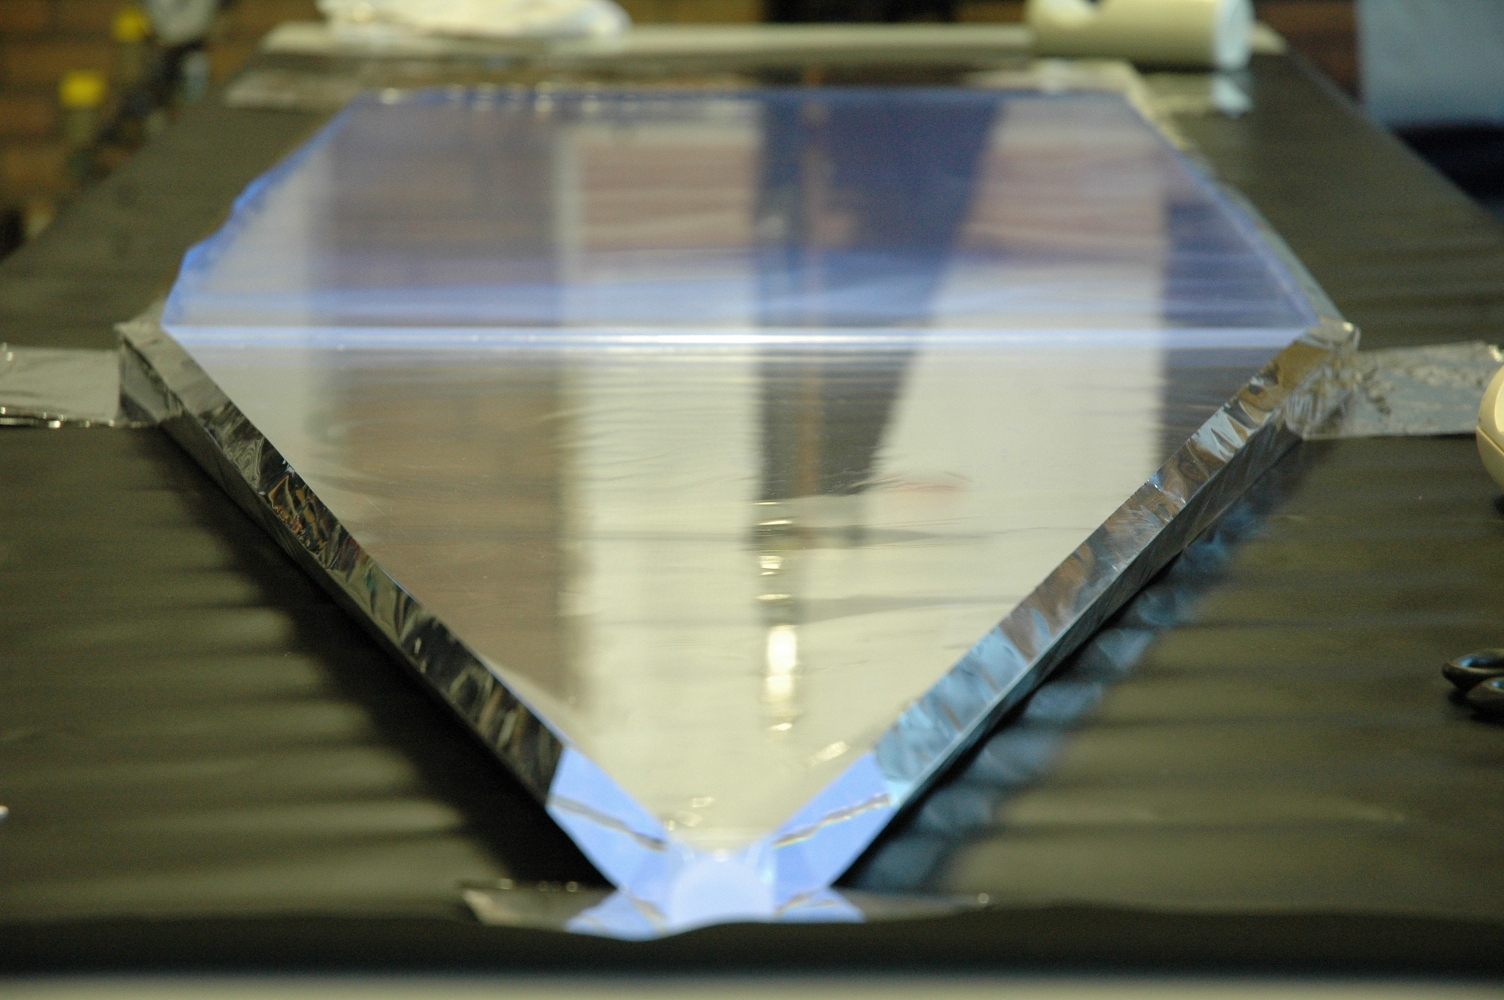
\includegraphics[scale=0.19]{DSC_0081a.eps}%
\caption{A partially wrapped light guided glued to the scintillator plate (back). }\label{fig:light_guide}
\end{center}\end{figure}

The photons are created by a process called fluorescence. A part of the energy of a passing particle is used to bring atoms inside the scintillating plate from their ground state to an excited state. These atoms would much rather be in their ground state. To return to this state they expel their excess energy in the form of a photon, light.

The scintillating plate is so sensitive that even visible and ultraviolet light can excite the atoms. The PMT is also sensitive to this light. For these reasons the HiSPARC detector is carefully wrapped in light tight plastic to prevent any light from entering. Even the tiniest leak can spoil the measurements.

In an ideal case the signal of the PMT is only dependent on the type of particle passing through the scintillating plate and not on the location of impact. The PMTs used by HiSPARC have a viewing window of a few square centimetres, much smaller than the size of our plates. It therefore stands to reason that if we were to attach the PMT directly to the plate, photons created near to the PMT have a much higher chance of being captured by the PMT than photons created at the other end of the plate. To reduce this unwanted effect a light guide is used to connect the PMT to the scintillating plate.

\section{Theoretical Evaluation of the Detector}
A simple schematic representation of the scintillator plate with the light guide attached would be a rectangle with a triangle attached to one of the shorter sides, both of equal thickness.\footnote{The actual shape and thickness of the light guide is a bit different to make the construction process easier and more forgiving to small mistakes.} All surfaces all carefully polished. As long as the angle of incidence is larger than the critical angle, total internal reflection by these surfaces will keep the light created by fluorescence inside the scintillating plate and/or light guide. This is illustrated in figure~\ref{fig:light_loss}.

\begin{figure}\begin{center}
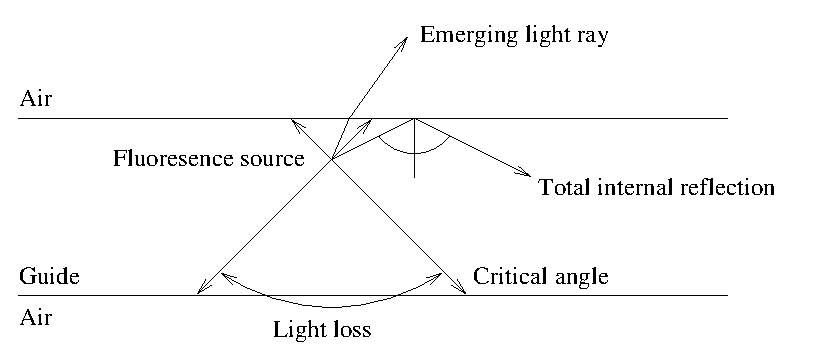
\includegraphics[scale=1]{light_loss.eps}%
\caption{Loss of light in the light guide.}\label{fig:light_loss}
\end{center}\end{figure}

This figure also shows that some light is lost because the created light spreads into all directions. To minimise this loss of light both the plate and guide are wrapped in aluminium foil. This foil acts like a mirror reflecting the light back into the detector. However, with each reflection a part of the light is absorbed, so we still lose some light here. For now we will keep matters simple and only look at the light contained by total internal reflection.

A passing particle will create a fluorescent line across the entire thickness of the scintillating. We only showed one point of this line in figure~\ref{fig:light_loss}. This figure shows that, for every location inside the light guide and scintillator plate the light loss in the vertical direction is the same.

The light created by the particles spread throughout the entire detector and reaches the PMT. In the module `The Universe' we explained how the apparent brightness (called apparent magnitude in astronomy) is inversely proportional to the distance squared. Does this law also apply to our detector?

\begin{shaded}
\textbf{Exercise \theExercise \stepcounter{Exercise}} : The module `The Universe' uses ever larger cubes to explain how light spreads out. The surface area of these cubes increases when we increase the length of their sides, thereby decreasing the brightness. However, in our detector the surface area is fixed. Light which is not lost can be seen as spreading out along cylinders. 

Show that the light intensity in our detector is inversely proportional to the distance. \end{shaded}

A top view of our HiSPARC detector can be seen in figure~\ref{fig:top_view}. At first glance it may seem as though the amount of light (per unit area) increases as we come nearer to the position of the PMT (right most part of the detector, not drawn in the figure) because the light guide gets smaller. In the figure we have drawn the location where the cosmic particle hits our detector and a few rays of light created by this event. Of course the light is not restrained to these five lines but spreads out into all directions. A part of the light travels in a straight line to the PMT, other rays may need to be reflected a few times while others might never reach the PMT.

\begin{figure}\begin{center}
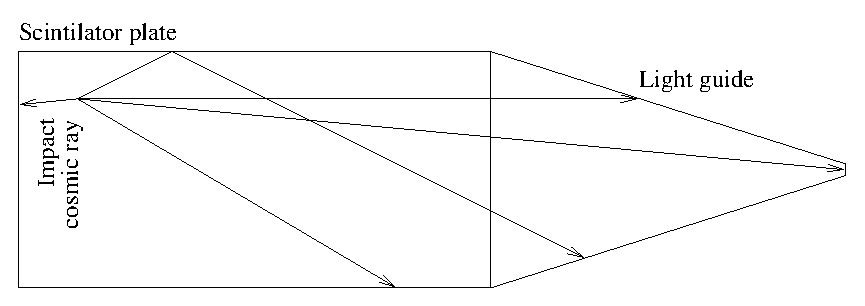
\includegraphics[scale=1]{top_view.eps}
\caption{Top view of the detector.}\label{fig:top_view}
\end{center}\end{figure}

\begin{shaded}
\textbf{Exercise \theExercise \stepcounter{Exercise}} : Complete the paths of the four rays of light not directly headed for the PMT in figure~\ref{fig:top_view} and show whether or not they reach the PMT. How does the light guide influence the (paths of the) rays? \end{shaded}

Figure~\ref{fig:top_view} is not the most convenient tool to answer the question how much light reaches the PMT. We would need to draw a lot of rays and still we would only have a rough estimation. If we are only interested in a rough estimation we can use a different, more simplified model. Figure~\ref{fig:top_view_simp} shows this new model. Our triangular light guide is replaced by a rectangular one. Three rays are drawn in this figure. One going directly to the PMT, the other two are reflected once before going to the PMT. Suppose these were drawn at exactly the critical angle.

\begin{figure}\begin{center}
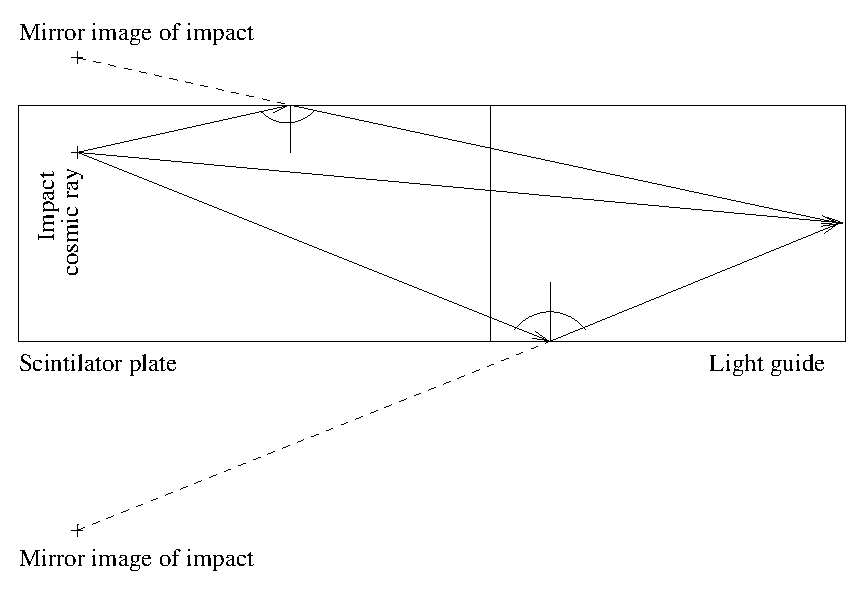
\includegraphics[scale=1]{top_view_simp.eps}
\caption{Top view of the detector showing two mirror images of the impact site.}\label{fig:top_view_simp}
\end{center}\end{figure}

\begin{shaded}
\textbf{Exercise \theExercise \stepcounter{Exercise}} : Explain how the demands for total internal reflection limit the number of reflections.\end{shaded}
\begin{shaded}
\textbf{Exercise \theExercise \stepcounter{Exercise}} : Explain how the amount of light rays reaching the PMT increases as the distance between the point of impact and the PMT increases.\end{shaded}

Our new model allows us to make the following assumptions:
\begin{itemize}
\item The intensity of the beam of light is inversely proportional to the distance.
\item The number of beams of light that can be detected by the PMT is directly proportional to the distance.
\end{itemize}
If both assumptions are valid then the point of impact does not influence the measured signal from the PMT.

\begin{shaded}
\textbf{Exercise \theExercise \stepcounter{Exercise}} : Argue whether or not our new model is valid.\end{shaded}

\section{A Practical Simulation}
Our theories about how the detector reflects and measures light can be tested using an experimental setup like the one in figure~\ref{fig:exp_setup}. A water tank is used as a model for our plastic plates. Waves in the water represent light waves. Besides the water tank we need two triangular pieces of plastic and a dropping pipette. We can drop small droplets of water in either side of the tank, either simulating our true detector or our simplified model.

The energy of the falling droplet creates waves in the water which spread across the entire surface. The wave collides with the sides of the tank and inserts. Like the light in the detector it is reflected (and a part is absorbed). The waves passing through the opening into the other compartment can be compared to the light detected by the PMT.

\begin{shaded}
\textbf{Exercise \theExercise \stepcounter{Exercise}} : When the angle of incidence is smaller than the critical angle there is no (total) reflection. Sadly our water tank model does not account for this. How can this form of absorption or light loss be incorporated into the experimental model? \end{shaded}

\begin{figure}[h]\begin{center}
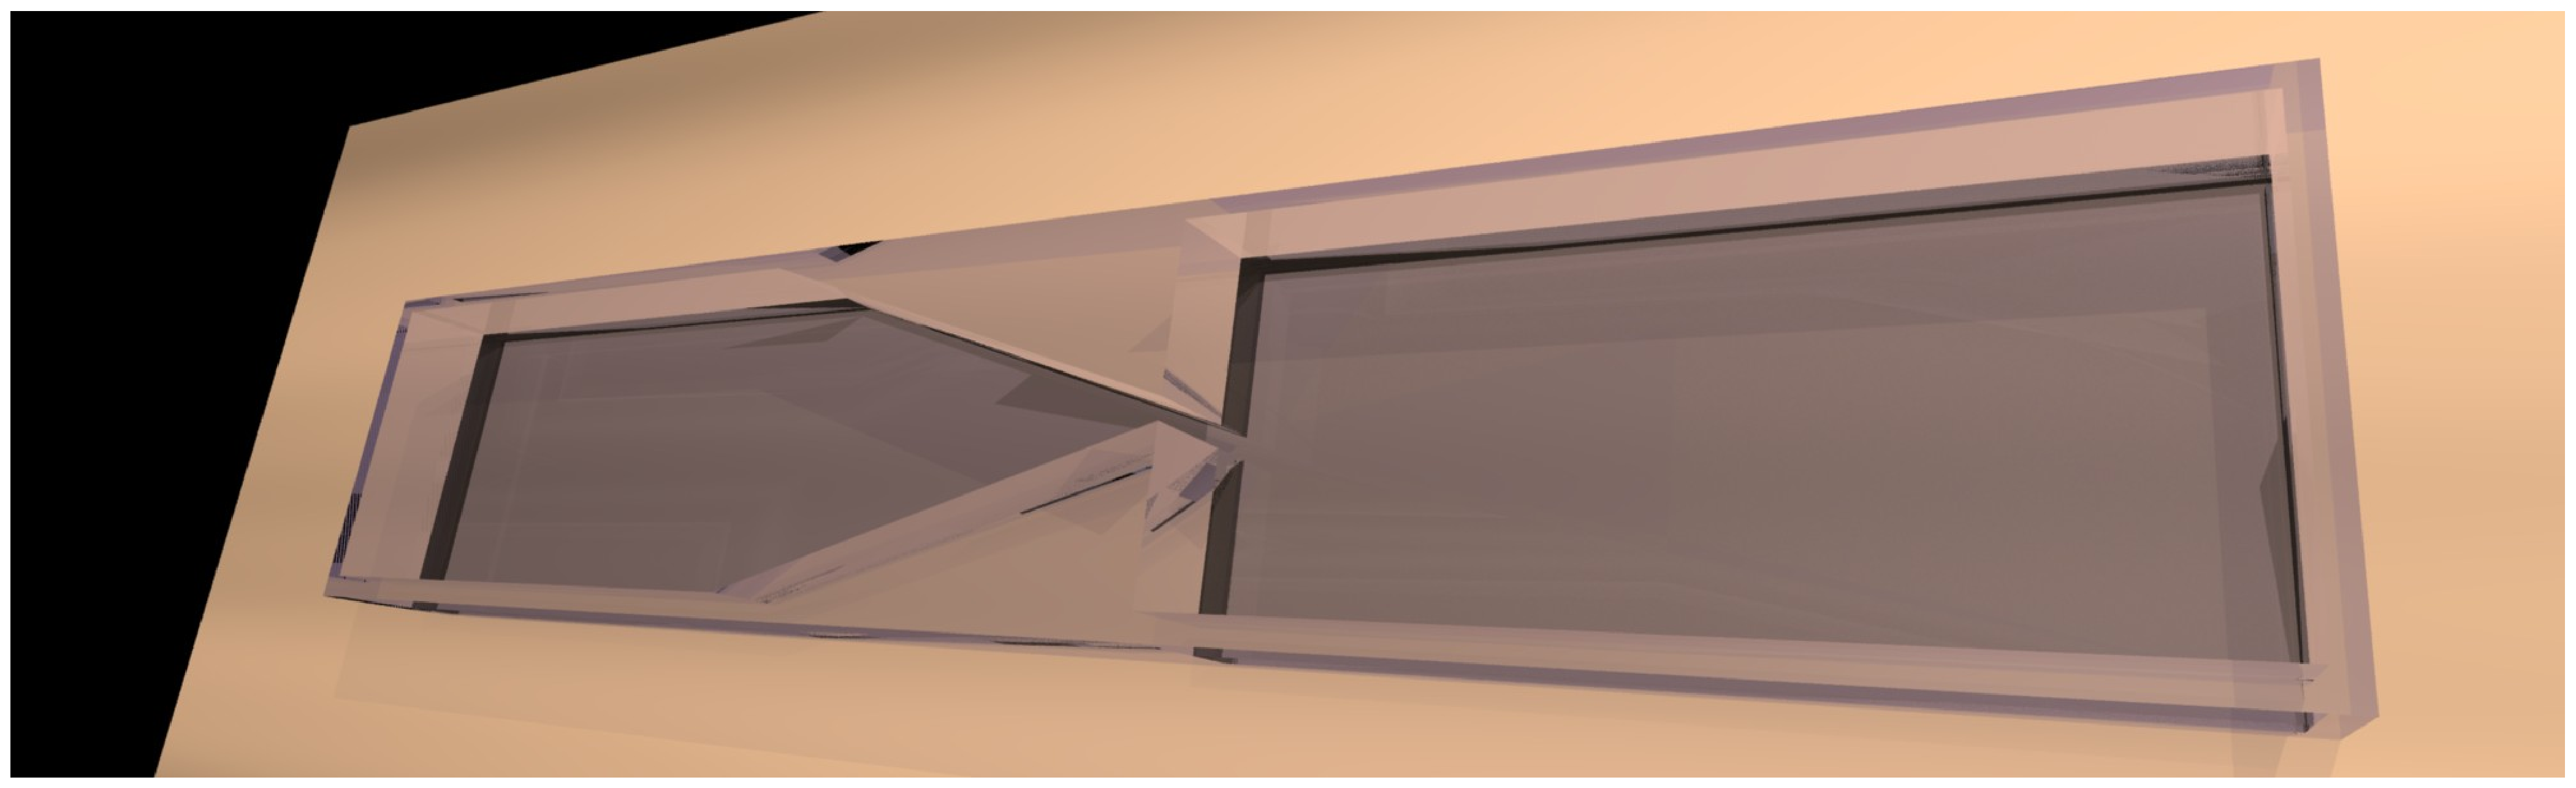
\includegraphics[scale=0.22]{simulatie4.eps}
\caption{Setup to simulate the HiSPARC detector.}\label{fig:exp_setup}
\end{center}\end{figure}

\end{document}

